\documentclass{article}

\usepackage{polski}
\usepackage{amsmath}
\usepackage{graphicx}
\usepackage{float}
\usepackage{subfig}
\usepackage{multirow}

\title{Rozwiązywanie równań i układów równań nieliniowych}
\author{\textbf{Łukasz Wala}\\
    \textit{AGH, Wydział Informatyki, Elektroniki i Telekomunikacji} \\
    \textit{Metody Obliczeniowe w Nauce i Technice 2021/2022}}
\date{Kraków, \today}

\begin{document}
\maketitle

\section{Problem 1}
\subsection{Opis problemu}
Główną ideą zadanie jest wyznaczenie pierwiastków równania $f(x)=0$ w zadanym przedziale metodą Newtona oraz metodą siecznych.
Dla metody Newtona punkty startowe wybierane będą rozpoczynając od wartości końców przedziału, zmniejszając je o 0.1 w kolejnych eksperymentach numerycznych.
Odpowiednio dla metody siecznej jeden z końców przedziału stanowić powinna wartość punktu startowego dla 
metody Newtona, a drugi - początek, a następnie koniec przedziału [a, b].

Badana funkcja:
\[f(x)=mxe^{-n}-me^{-nx}+1/m\]
Gdzie $n=9$, $m=25$ oraz $x\in [0.1,1.9]$.

Liczba iteracji dla obu tych metod (dla różnych dokładności $\rho$) zostanie porównana, stosując kryteria stopu:
\begin{enumerate}
    \item 
    $\left|x_{(i+1)}-x_{(i)}\right| < \rho$
    \item
    $\left|f(x_i)\right| < \rho$
\end{enumerate}

\subsection{Opracowanie}
Wykres badanej funkcji wygląda następująco:

\begin{figure}[H]
    \centering
    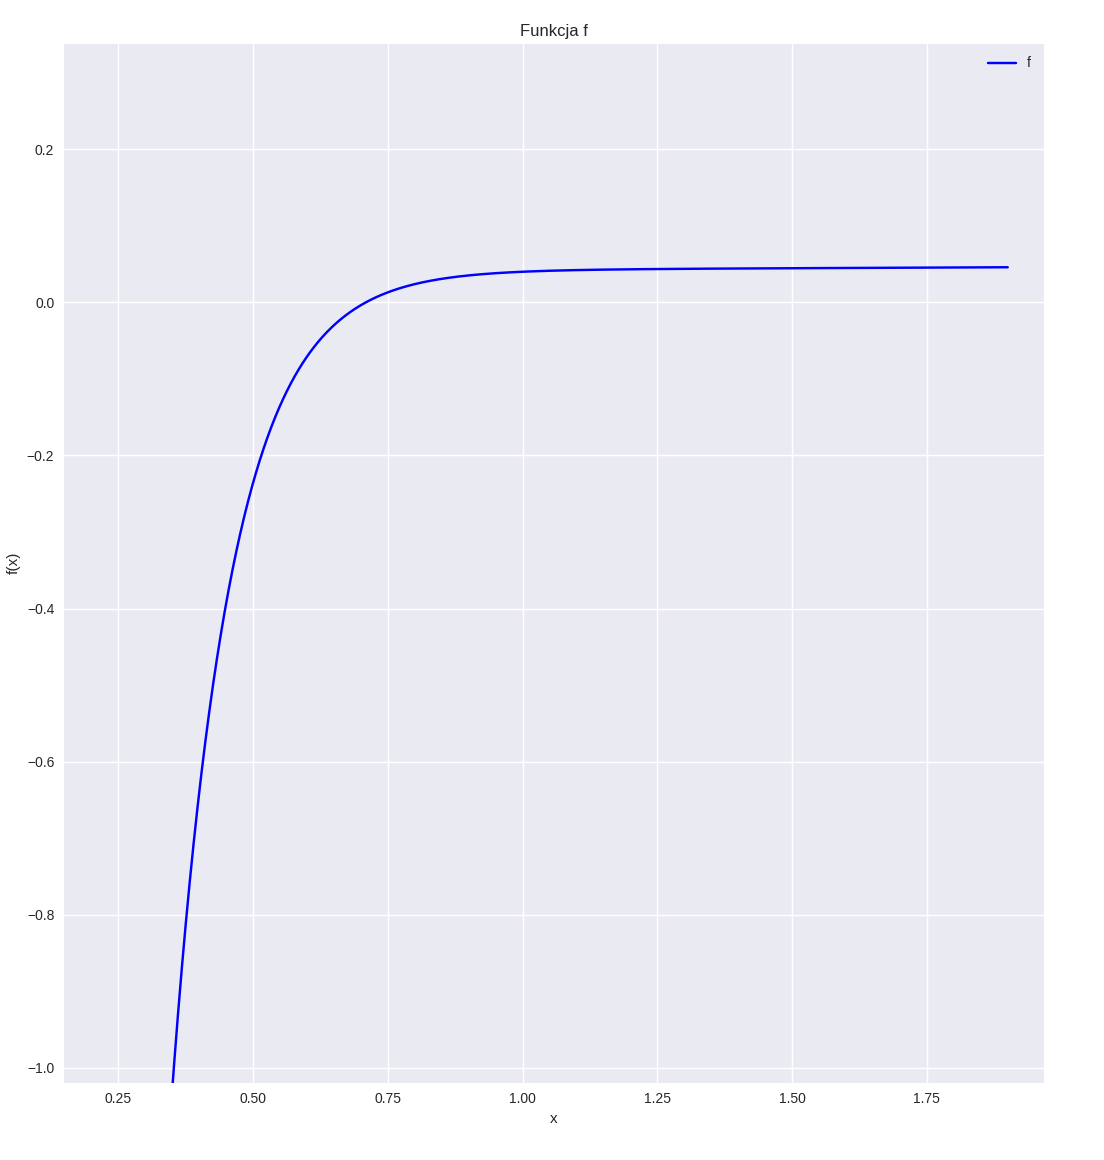
\includegraphics[width=\textwidth]{img/funkcja.png}
    \caption{Funkcja $f$}
\end{figure}

Już na jego podstawie można przewidywać, że miejsce zerowe funkcji znajduje się w okolicach $x=0.7$ .

\subsubsection{Metoda Newtona}
Obie metody zaimplementowane zostały w języku Python.
W metodzie Newtona konieczna jest znajomość pochodnej funkcji $f$, zostanie ona wyznaczona analitycznie:

$$f'(x)=me^{(-n)} + nme^{(-nx)}$$

Żeby zastosować metodę Newtona muszą być spełnione warunki:
\begin{enumerate}
    \item
    funkcja jest ciągła,
    \item 
    w przedziale znajduje się dokładnie jeden pierwiastek,
    \item
    funkcja ma różne znaki na krańcach przedziału,
    \item
    pierwsza i druga pochodna funkcji mają stały znak w tym przedziale.
\end{enumerate}

W przypadku funkcji $f$ wszystkie warunki są spełnione.

Poniżej znajdują się tabele z wynikami oraz liczbami iteracji dla różnych punktów startowych, dokładności i kryteriów stopu
(kolumny - dokładność $\rho$, wiersze - punkt startowy):

\begin{table}[H]
\centering
\begin{tabular}{|l|l|l|l|l|l|}
\hline
& 0.01 & 0.001 & 0.0001 & 0.00001 & 0.000001 \\ \hline
1.90 & 126 & 127 & 128 & 128 & 128 \\ \hline
1.80 & 126 & 127 & 127 & 127 & 128 \\ \hline
1.70 & 124 & 125 & 126 & 126 & 126 \\ \hline
1.60 & 121 & 122 & 123 & 123 & 123 \\ \hline
1.50 & 115 & 116 & 116 & 116 & 117 \\ \hline
1.40 & 101 & 102 & 102 & 103 & 103 \\ \hline
1.30 & 78 & 79 & 79 & 80 & 80 \\ \hline
1.20 & 50 & 51 & 51 & 51 & 52 \\ \hline
1.10 & 26 & 27 & 28 & 28 & 28 \\ \hline
1.00 & 13 & 13 & 14 & 14 & 15 \\ \hline
0.90 & 6 & 7 & 8 & 8 & 8 \\ \hline
0.80 & 3 & 4 & 5 & 5 & 5 \\ \hline
0.70 & 1 & 2 & 3 & 3 & 3 \\ \hline
0.60 & 3 & 4 & 5 & 5 & 5 \\ \hline
0.50 & 4 & 5 & 6 & 6 & 6 \\ \hline
0.40 & 5 & 6 & 7 & 7 & 7 \\ \hline
0.30 & 6 & 7 & 8 & 8 & 8 \\ \hline
0.20 & 7 & 8 & 8 & 9 & 9 \\ \hline
0.10 & 8 & 9 & 9 & 10 & 10 \\ \hline
\end{tabular}
\caption{Liczba iteracji dla kryterium 1}
\end{table}

\begin{table}[H]
\centering
\begin{tabular}{|l|l|l|l|l|l|}
\hline
& 0.01 & 0.001 & 0.0001 & 0.00001 & 0.000001 \\ \hline
1.90 & 125 & 126 & 126 & 127 & 127 \\ \hline
1.80 & 124 & 125 & 126 & 126 & 127 \\ \hline
1.70 & 123 & 124 & 125 & 125 & 125 \\ \hline
1.60 & 120 & 121 & 122 & 122 & 122 \\ \hline
1.50 & 113 & 114 & 115 & 115 & 116 \\ \hline
1.40 & 99 & 100 & 101 & 101 & 102 \\ \hline
1.30 & 76 & 77 & 78 & 78 & 79 \\ \hline
1.20 & 48 & 49 & 50 & 50 & 51 \\ \hline
1.10 & 25 & 26 & 27 & 27 & 27 \\ \hline
1.00 & 11 & 12 & 13 & 13 & 13 \\ \hline
0.90 & 5 & 6 & 6 & 7 & 7 \\ \hline
0.80 & 2 & 3 & 4 & 4 & 4 \\ \hline
0.70 & 1 & 1 & 2 & 2 & 2 \\ \hline
0.60 & 2 & 3 & 3 & 4 & 4 \\ \hline
0.50 & 3 & 4 & 4 & 5 & 5 \\ \hline
0.40 & 4 & 5 & 5 & 6 & 6 \\ \hline
0.30 & 5 & 6 & 6 & 7 & 7 \\ \hline
0.20 & 6 & 7 & 7 & 8 & 8 \\ \hline
0.10 & 7 & 8 & 8 & 9 & 9 \\ \hline
\end{tabular}
\caption{Liczba iteracji dla kryterium 2}
\end{table}

Nietrudno zauważyć, że niezależnie o warunku, metoda Newtona potrzebuje tym więcej iteracji, im dalej znajduje się od
pierwiastka, z tym, że iteracji przybywa znacznie szybciej w stronę prawego krańca przedziału. Jest to spowodowane faktem, że dla większych $x$ funkcja się wypłaszcza, przez co pierwsza styczna
jest prawie równoległa z osią X (dla $1.9$ punkt przecięcia pierwszej stycznej to ok. $-12$). Dla ujemnych lub bardzo małych
$x$ funkcja natomiast jest bardzo stroma, więc każda iteracja daje niewielki postęp ku pierwiastkowi. Dokładność
nie ma dużego wpływu na liczbę iteracji.

\begin{table}[H]
\centering
\begin{tabular}{|l|l|l|l|l|l|}
\hline
& 0.01 & 0.001 & 0.0001 & 0.00001 & 0.000001 \\ \hline
1.90 & 0.709233 & 0.70938659 & 0.709386700 & 0.70938670074244 & 0.70938670074244 \\ \hline
1.80 & 0.709380 & 0.70938670 & 0.709386700 & 0.70938670057208 & 0.70938670074249 \\ \hline
1.70 & 0.708984 & 0.70938597 & 0.709386700 & 0.70938670074017 & 0.70938670074017 \\ \hline
1.60 & 0.708979 & 0.70938596 & 0.709386700 & 0.70938670074006 & 0.70938670074006 \\ \hline
1.50 & 0.709381 & 0.70938670 & 0.709386700 & 0.70938670063318 & 0.70938670074249 \\ \hline
1.40 & 0.709365 & 0.70938669 & 0.709386698 & 0.70938670074249 & 0.70938670074249 \\ \hline
1.30 & 0.709371 & 0.70938669 & 0.709386699 & 0.70938670074249 & 0.70938670074249 \\ \hline
1.20 & 0.709377 & 0.70938670 & 0.709386700 & 0.70938670035667 & 0.70938670074249 \\ \hline
1.10 & 0.709047 & 0.70938618 & 0.709386700 & 0.70938670074132 & 0.70938670074132 \\ \hline
1.00 & 0.709384 & 0.70938426 & 0.709386700 & 0.70938670071595 & 0.70938670074249 \\ \hline
0.90 & 0.709247 & 0.70938661 & 0.709386700 & 0.70938670074246 & 0.70938670074246 \\ \hline
0.80 & 0.709021 & 0.70938610 & 0.709386700 & 0.70938670074092 & 0.70938670074092 \\ \hline
0.70 & 0.709003 & 0.70938604 & 0.709386700 & 0.70938670074059 & 0.70938670074059 \\ \hline
0.60 & 0.709214 & 0.70938656 & 0.709386700 & 0.70938670074241 & 0.70938670074241 \\ \hline
0.50 & 0.709148 & 0.70938644 & 0.709386700 & 0.70938670074221 & 0.70938670074221 \\ \hline
0.40 & 0.709193 & 0.70938653 & 0.709386700 & 0.70938670074237 & 0.70938670074237 \\ \hline
0.30 & 0.709256 & 0.70938662 & 0.709386700 & 0.70938670074247 & 0.70938670074247 \\ \hline
0.20 & 0.709306 & 0.70938667 & 0.709386672 & 0.70938670074249 & 0.70938670074249 \\ \hline
0.10 & 0.709340 & 0.70938669 & 0.709386691 & 0.70938670074249 & 0.70938670074249 \\ \hline
\end{tabular}
\caption{Wyniki dla warunku 1}
\end{table}

Mniejsza wartość $\rho$ skutkuje większą liczbą cyfr niezmiennych (tj. takich, które nie zmieniają się w zależności od punkut startowego).

\begin{table}[H]
\centering
\begin{tabular}{|l|l|l|l|l|l|}
\hline
& 0.01 & 0.001 & 0.0001 & 0.00001 & 0.000001 \\ \hline
1.90 & 0.703480 & 0.70923364 & 0.709233642 & 0.709386596 & 0.70938659621 \\ \hline
1.80 & 0.692741 & 0.70820814 & 0.709380522 & 0.709380522 & 0.70938670057 \\ \hline
1.70 & 0.699758 & 0.70898435 & 0.709385979 & 0.709385979 & 0.70938597900 \\ \hline
1.60 & 0.699701 & 0.70897963 & 0.709385961 & 0.709385961 & 0.70938596197 \\ \hline
1.50 & 0.693662 & 0.70833216 & 0.709381752 & 0.709381752 & 0.70938670063 \\ \hline
1.40 & 0.686576 & 0.70721198 & 0.709365723 & 0.709365723 & 0.70938669877 \\ \hline
1.30 & 0.688373 & 0.70753170 & 0.709371424 & 0.709371424 & 0.70938669970 \\ \hline
1.20 & 0.690898 & 0.70794044 & 0.709377403 & 0.709377403 & 0.70938670035 \\ \hline
1.10 & 0.700560 & 0.70904775 & 0.709386188 & 0.709386188 & 0.70938618844 \\ \hline
1.00 & 0.696264 & 0.70864681 & 0.709384262 & 0.709384262 & 0.70938426244 \\ \hline
0.90 & 0.703759 & 0.70924766 & 0.709247665 & 0.709386614 & 0.70938661448 \\ \hline
0.80 & 0.700223 & 0.70902175 & 0.709386106 & 0.709386106 & 0.70938610687 \\ \hline
0.70 & 0.709003 & 0.70900399 & 0.709386047 & 0.709386047 & 0.70938604770 \\ \hline
0.60 & 0.703113 & 0.70921421 & 0.709214213 & 0.709386568 & 0.70938656800 \\ \hline
0.50 & 0.702006 & 0.70914872 & 0.709148723 & 0.709386448 & 0.70938644812 \\ \hline
0.40 & 0.702742 & 0.70919343 & 0.709193437 & 0.709386534 & 0.70938653411 \\ \hline
0.30 & 0.703940 & 0.70925636 & 0.709256364 & 0.709386624 & 0.70938662494 \\ \hline
0.20 & 0.705125 & 0.70930666 & 0.709306664 & 0.709386672 & 0.70938667215 \\ \hline
0.10 & 0.706154 & 0.70934050 & 0.709340505 & 0.709386691 & 0.70938669121 \\ \hline
\end{tabular}
\caption{Wyniki dla warunku 2}
\end{table}

Zastosowanie drugiego kryterium stopu daje natomiast mniej dokładne wyniku dla takiej samej wartości $\rho$
(mniejsza liczba cyfr nizmiennych niezależnie od punktu startowego).

\subsubsection{Metoda siecznych}
Żeby zastosować metodę siecznych muszą być spełnione warunki:
\begin{enumerate}
    \item
    funkcja jest ciągła,
    \item
    funkcja ma różne znaki na krańcach przedziału,
\end{enumerate}

Pierwszą przewagą metody siecznych nad metodą Newtona jest mniejsza liczba warunków oraz fakt, że pochodna nie musi być znana.

Poniżej tabele z iteracjami i dokładnościami (analogicznie jak w przypadku metody Newtona):

\begin{table}[H]
\centering
\begin{tabular}{|l|l|l|l|l|l|}
\hline
& 0.01 & 0.001 & 0.0001 & 0.00001 & 0.000001 \\ \hline
[0.10, 1.90] & 1 & 270 & 377 & 474 & 570 \\ \hline
[0.10, 1.80] & 1 & 257 & 364 & 461 & 558 \\ \hline
[0.10, 1.70] & 1 & 243 & 351 & 448 & 544 \\ \hline
[0.10, 1.60] & 1 & 229 & 336 & 433 & 529 \\ \hline
[0.10, 1.50] & 1 & 213 & 321 & 418 & 514 \\ \hline
[0.10, 1.40] & 1 & 196 & 304 & 401 & 497 \\ \hline
[0.10, 1.30] & 1 & 178 & 285 & 382 & 478 \\ \hline
[0.10, 1.20] & 1 & 158 & 265 & 362 & 458 \\ \hline
[0.10, 1.10] & 1 & 135 & 242 & 339 & 436 \\ \hline
[0.10, 1.00] & 1 & 109 & 217 & 314 & 410 \\ \hline
[0.10, 0.90] & 1 & 78 & 185 & 282 & 378 \\ \hline
[0.10, 0.80] & 1 & 33 & 140 & 237 & 334 \\ \hline
[0.10, 0.70] & 2 & 3 & 4 & 5 & 5 \\ \hline
[0.10, 0.60] & 4 & 7 & 10 & 12 & 15 \\ \hline
[0.10, 0.50] & 6 & 12 & 17 & 23 & 28 \\ \hline
[0.10, 0.40] & 9 & 19 & 30 & 42 & 53 \\ \hline
[0.10, 0.30] & 11 & 30 & 53 & 76 & 99 \\ \hline
[0.10, 0.20] & 13 & 46 & 92 & 139 & 186 \\ \hline
\end{tabular}
\caption{Liczba iteracji dla kryterium 1}
\end{table}

\begin{table}[H]
\centering
\begin{tabular}{|l|l|l|l|l|l|}
\hline
& 0.01 & 0.001 & 0.0001 & 0.00001 & 0.000001 \\ \hline
[0.10, 1.90] & 292 & 396 & 493 & 589 & 685 \\ \hline
[0.10, 1.80] & 279 & 384 & 480 & 577 & 673 \\ \hline
[0.10, 1.70] & 266 & 370 & 467 & 563 & 659 \\ \hline
[0.10, 1.60] & 251 & 356 & 452 & 548 & 645 \\ \hline
[0.10, 1.50] & 235 & 340 & 437 & 533 & 629 \\ \hline
[0.10, 1.40] & 218 & 323 & 420 & 516 & 612 \\ \hline
[0.10, 1.30] & 200 & 305 & 401 & 498 & 594 \\ \hline
[0.10, 1.20] & 180 & 284 & 381 & 477 & 573 \\ \hline
[0.10, 1.10] & 157 & 262 & 359 & 455 & 551 \\ \hline
[0.10, 1.00] & 131 & 236 & 333 & 429 & 525 \\ \hline
[0.10, 0.90] & 100 & 204 & 301 & 397 & 493 \\ \hline
[0.10, 0.80] & 55 & 160 & 257 & 353 & 449 \\ \hline
[0.10, 0.70] & 1 & 2 & 3 & 3 & 4 \\ \hline
[0.10, 0.60] & 3 & 5 & 8 & 11 & 13 \\ \hline
[0.10, 0.50] & 6 & 11 & 17 & 22 & 28 \\ \hline
[0.10, 0.40] & 11 & 22 & 33 & 44 & 55 \\ \hline
[0.10, 0.30] & 21 & 43 & 66 & 88 & 111 \\ \hline
[0.10, 0.20] & 42 & 86 & 133 & 180 & 227 \\ \hline
\end{tabular}
\caption{Liczba iteracji dla kryterium 2}
\end{table}

Dla warunku 1 przy $\rho = 0.01$ prawdopodobnie występuje błąd, zostanie to potwierdzone przy tabelach z wynikami,
Widać również wyraźny spadek liczby iteracji gdy początek przedziału staje się równy 0.7, jest to oczywiście spowodowane faktem,
że przy takiej konfiguracji pierwiastek nie znajduje się już w przedziale i założenia metody nie są spełnione.

\begin{table}[H]
\centering
\begin{tabular}{|l|l|l|l|l|l|}
\hline
& 0.01 & 0.001 & 0.0001 & 0.00001 & 0.000001 \\ \hline
[0.10, 1.90] & 1 & 270 & 377 & 474 & 570 \\ \hline
[0.20, 1.90] & 54 & 139 & 186 & 230 & 273 \\ \hline
[0.30, 1.90] & 45 & 70 & 89 & 108 & 126 \\ \hline
[0.40, 1.90] & 26 & 32 & 36 & 38 & 67 \\ \hline
[0.50, 1.90] & 14 & 18 & 27 & 59 & 90 \\ \hline
[0.60, 1.90] & 12 & 14 & 47 & 80 & 114 \\ \hline
[0.70, 1.90] & 5 & 14 & 21 & 29 & 35 \\ \hline
\end{tabular}
\caption{Liczba iteracji dla kryterium 1}
\end{table}

\begin{table}[H]
\centering
\begin{tabular}{|l|l|l|l|l|l|}
\hline
& 0.01 & 0.001 & 0.0001 & 0.00001 & 0.000001 \\ \hline
[0.10, 1.90] & 292 & 396 & 493 & 589 & 685 \\ \hline
[0.20, 1.90] & 131 & 179 & 223 & 267 & 311 \\ \hline
[0.30, 1.90] & 59 & 79 & 98 & 116 & 134 \\ \hline
[0.40, 1.90] & 25 & 31 & 33 & 58 & 92 \\ \hline
[0.50, 1.90] & 11 & 15 & 49 & 81 & 112 \\ \hline
[0.60, 1.90] & 4 & 37 & 72 & 105 & 139 \\ \hline
[0.70, 1.90] & 5 & 14 & 21 & 28 & 35 \\ \hline
\end{tabular}
\caption{Liczba iteracji dla kryterium 2}
\end{table}

Przy zmnieniającym się początku przedziału po przekroczeniu $x$ równemu pierwiastkowi rutyna wpada w nieskńczoną pętlę, 
wyniku nie można otrzymać, z tego samego powodu, który jest opisany powyżej.

\begin{table}[H]
\centering
\begin{tabular}{|l|l|l|l|l|l|}
\hline
& 0.01 & 0.001 & 0.0001 & 0.00001 & 0.000001 \\ \hline
[0.10, 1.90] & 1.9 & 0.757249 & 0.71361 & 0.7098050 & 0.709428616 \\ \hline
[0.10, 1.80] & 1.799 & 0.7575 & 0.71364 & 0.7098082 & 0.709427939 \\ \hline
[0.10, 1.70] & 1.699 & 0.7580 & 0.71359 & 0.7098028 & 0.709428396 \\ \hline
[0.10, 1.60] & 1.599 & 0.7575 & 0.71364 & 0.7098076 & 0.709428883 \\ \hline
[0.10, 1.50] & 1.499 & 0.7578 & 0.71358 & 0.7098013 & 0.709428252 \\ \hline
[0.10, 1.40] & 1.399 & 0.7579 & 0.71358 & 0.7098022 & 0.709428336 \\ \hline
[0.10, 1.30] & 1.299 & 0.7575 & 0.71364 & 0.7098079 & 0.709428907 \\ \hline
[0.10, 1.20] & 1.199 & 0.7572 & 0.71361 & 0.7098052 & 0.709428640 \\ \hline
[0.10, 1.10] & 1.099 & 0.7576 & 0.71365 & 0.7098092 & 0.709428041 \\ \hline
[0.10, 1.00] & 0.999 & 0.7577 & 0.71357 & 0.7098005 & 0.709428167 \\ \hline
[0.10, 0.90] & 0.899 & 0.7574 & 0.71363 & 0.7098068 & 0.709428796 \\ \hline
[0.10, 0.80] & 0.799 & 0.7576 & 0.71365 & 0.7098092 & 0.709428038 \\ \hline
[0.10, 0.70] & 0.699 & 0.6999 & 0.69999 & 0.6999999 & 0.699999999 \\ \hline
[0.10, 0.60] & 0.599 & 0.5999 & 0.59999 & 0.5999999 & 0.599999999 \\ \hline
[0.10, 0.50] & 0.499 & 0.4999 & 0.49999 & 0.4999999 & 0.499999999 \\ \hline
[0.10, 0.40] & 0.399 & 0.3999 & 0.39999 & 0.3999999 & 0.399999999 \\ \hline
[0.10, 0.30] & 0.299 & 0.2999 & 0.29999 & 0.2999999 & 0.299999999 \\ \hline
[0.10, 0.20] & 0.199 & 0.1999 & 0.19999 & 0.1999999 & 0.199999999 \\ \hline
\end{tabular}
\caption{Wyniki dla warunku 1}
\end{table}

\begin{table}[H]
\centering
\begin{tabular}{|l|l|l|l|l|l|}
\hline
& 0.01 & 0.001 & 0.0001 & 0.00001 & 0.000001 \\ \hline
[0.10, 1.90] & 0.73930 & 0.712081 & 0.709652 & 0.7094132 & 0.709389361 \\ \hline
[0.10, 1.80] & 0.73951 & 0.712038 & 0.709654 & 0.7094128 & 0.709389318 \\ \hline
[0.10, 1.70] & 0.73916 & 0.712067 & 0.709650 & 0.7094131 & 0.709389347 \\ \hline
[0.10, 1.60] & 0.73947 & 0.712035 & 0.709653 & 0.7094134 & 0.709389314 \\ \hline
[0.10, 1.50] & 0.73972 & 0.712058 & 0.709649 & 0.7094130 & 0.709389337 \\ \hline
[0.10, 1.40] & 0.73977 & 0.712064 & 0.709650 & 0.7094131 & 0.709389343 \\ \hline
[0.10, 1.30] & 0.73949 & 0.712036 & 0.709653 & 0.7094128 & 0.709389316 \\ \hline
[0.10, 1.20] & 0.73932 & 0.712083 & 0.709652 & 0.7094132 & 0.709389362 \\ \hline
[0.10, 1.10] & 0.73958 & 0.712045 & 0.709648 & 0.7094129 & 0.709389324 \\ \hline
[0.10, 1.00] & 0.73966 & 0.712053 & 0.709649 & 0.7094129 & 0.709389332 \\ \hline
[0.10, 0.90] & 0.73942 & 0.712093 & 0.709653 & 0.7094133 & 0.709389372 \\ \hline
[0.10, 0.80] & 0.73958 & 0.712045 & 0.709648 & 0.7094129 & 0.709389324 \\ \hline
[0.10, 0.70] & 0.69999 & 0.699999 & 0.699999 & 0.6999999 & 0.699999999 \\ \hline
[0.10, 0.60] & 0.59999 & 0.599999 & 0.599999 & 0.5999999 & 0.599999999 \\ \hline
[0.10, 0.50] & 0.49999 & 0.499999 & 0.499999 & 0.4999999 & 0.499999999 \\ \hline
[0.10, 0.40] & 0.39999 & 0.399999 & 0.399999 & 0.3999999 & 0.399999999 \\ \hline
[0.10, 0.30] & 0.29999 & 0.299999 & 0.299999 & 0.2999999 & 0.299999999 \\ \hline
[0.10, 0.20] & 0.19999 & 0.199999 & 0.199999 & 0.1999999 & 0.199999999 \\ \hline
\end{tabular}
\caption{Wyniki dla warunku 2}
\end{table}

Tutaj wyraźnie widoczne jest to samo zjawisko: po przekroczeniu przez jeden z końców $x$ równego pierwiastkowi
wyniki są całkowicie niepoprawne.

\begin{table}[H]
\centering
\begin{tabular}{|l|l|l|l|l|l|}
\hline
& 0.01 & 0.001 & 0.0001 & 0.00001 & 0.000001 \\ \hline
[0.10, 1.90] & 1.999 & 0.757 & 0.7136 & 0.70980 & 0.709428 \\ \hline
[0.20, 1.90] & 1.157 & 0.730 & 0.7112 & 0.70957 & 0.709406 \\ \hline
[0.30, 1.90] & 0.827 & 0.717 & 0.7102 & 0.70946 & 0.709394 \\ \hline
[0.40, 1.90] & 0.739 & 0.711 & 0.7095 & 0.70949 & 0.709401 \\ \hline
[0.50, 1.90] & 0.722 & 0.712 & 0.7107 & 0.70951 & 0.709400 \\ \hline
[0.60, 1.90] & 0.731 & 0.722 & 0.7108 & 0.70953 & 0.709401 \\ \hline
[0.70, 1.90] & 0.745 & 0.712 & 0.7097 & 0.70941 & 0.709390 \\ \hline
\end{tabular}
\caption{Wyniki dla warunku 1}
\end{table}

\begin{table}[H]
\centering
\begin{tabular}{|l|l|l|l|l|l|}
\hline
& 0.01 & 0.001 & 0.0001 & 0.00001 & 0.000001 \\ \hline
[0.10, 1.90] & 0.739 & 0.7120 & 0.70965 & 0.7094132 & 0.70938936 \\ \hline
[0.20, 1.90] & 0.739 & 0.7120 & 0.70965 & 0.7094132 & 0.70938932 \\ \hline
[0.30, 1.90] & 0.739 & 0.7122 & 0.70965 & 0.7094148 & 0.70938965 \\ \hline
[0.40, 1.90] & 0.749 & 0.7127 & 0.71011 & 0.7094139 & 0.70938942 \\ \hline
[0.50, 1.90] & 0.789 & 0.7222 & 0.70966 & 0.7094131 & 0.70938940 \\ \hline
[0.60, 1.90] & 0.877 & 0.7122 & 0.70964 & 0.7094143 & 0.70938943 \\ \hline
[0.70, 1.90] & 0.745 & 0.7126 & 0.70974 & 0.7094223 & 0.70939023 \\ \hline
\end{tabular}
\caption{Wyniki dla warunku 2}
\end{table}

Zgodnie z obserwacjami liczby iteracji, dla dokładności 0.01 (w przedziałach, gdzie założenie jest jeszcze spełnione)
dla warunku 1 występują istotne błędy (np. $x=1.99$ dla przedziału $[0.1, 1.9]$ z dokłądnością 0.01). Są one spowodowane
prawdopodobnie użytym kryterium stopu: dwie kolejne wartości są na tyle blisko siebie, że rutyna jest przerywana, pomimo 
że do pierwiestka jest jeszcze daleko.

\subsection{Porównanie i wnioski}

Na podstawie obliczonych wartości widać, że metoda Newtona praktycznie w każdym przypadku potrzebuje znaczniej mniejszej
liczby iteracji niż metoda siecznych, żeby osiągnąć tą samą dokładność, oraz jej wyniki są bardziej konsekwentne względem
punktu startowego. Należy jednak pamiętać, że do wykorzystania metody Newtona musi być spełnione więcej założeń, potrzebna
jest znajomość pochodnej funkcji oraz (co nie wystąpiło w tym przypadku) nie zawsze jest zbieżna do pierwiastka funkcji.
Stąd najlepiej jest stosować w połączeniu metodę Newtona oraz metodę siecznych lub bisekcji, gdy użycie metody Newtona z jakiegoś powodu
nie jest możliwe.

\section{Problem 2}
\subsection{Opis problemu}
Główną ideą problemu jest rozwiązanie układu równań metodą Newtona.
\[
\begin{cases}
    x^2_1+x^2_2-x^2_3=1 \\
    x_1-2x^3_2+2^2_3=-1 \\
    2x_1^2+x_2-2x^2_3=1
\end{cases}
\]

Eksperymenty zostaną przeprowadzone dla różnych wektorów początkowych. 
Sprawdzona zostanie liczba rozwiązań układu, przy jakich wektorach początkowych metoda 
nie zbiega do rozwiązania oraz to jakie wektory początkowe doprowadzają do jakiego 
rozwiązania. Zastosowane zostaną dwa różne kryteria stopu (analogiczne do problemu 1, normy euklidesowe):
\begin{enumerate}
    \item 
    $\left\|X_{(i+1)}-X_{(i)}\right\| < \rho$
    \item
    $\left\|F(X_i)\right\| < \rho$
\end{enumerate}

\subsection{Opracowanie}
Niech
$$F(X)=
\begin{bmatrix}
    f_1(X) \\
    f_2(X) \\
    f_3(X) \\
\end{bmatrix}
=
\begin{bmatrix}
    x^2_1+x^2_2-x^2_3 -1\\
    x_1-2x^3_2+2^2_3 +1\\
    2x_1^2+x_2-2x^2_3 -1\\
\end{bmatrix}
$$

Metoda Newtona dla układów równań jest analogiczna jak dla równania nieliniowego z tą różnicą, że zamiast pochodnej używany
jest jakobian macierzy, w tym przypadku:
$$J(X)=
\begin{bmatrix}
    2x_1 & 2x_2 & -2x_3 \\
    1 & -6x_2^2 & 4x_3 \\
    4x_1 & 1 & -4x_3 \\
\end{bmatrix}
$$
Wówczas
$$X_{k+1} = X_k - \frac{F(X_k)}{J(X_k)}$$
Czyli
$$X_{k+1} = X_k - J(X_k)^{-1}F(X_k)$$
Gdzie $J(X_k)^{-1}F(X_k)$ jest rozwiązaniem układu równań $J(X_k)S = F(X_k)$, więc
$$X_{k+1} = X_k - S$$

Program obliczający rozwiązanie układu napisany został w języku Python, układ równań rozwiązywany za pomocą numpy.linalg.solve().

Układ nie jest trudny do obliczenia metodami analitycznymi, ma on cztery rzeczywiste rozwiązania:
\begin{itemize}
    \item 
    $x_1= -1, x_2= 1, x_3= -1$
    \item 
    $x_1= -1, x_2= 1, x_3= 1$
    \item 
    $x_1= \frac{1}{2}, x_2= 1, x_3= -\frac{1}{2}$
    \item 
    $x_1= \frac{1}{2}, x_2= 1, x_3= \frac{1}{2}$
\end{itemize}

W metodzie Newtona rozważane były wektory początkowe z przedziału [-1,-1,-1] do [1,1,1] indywidualnie dla każdej współrzędnej, 
w różnych kombinacjach. Taki wybór uzasadniony jest faktem, że w tym przedziale znajdują się wszystkie rozwiązania oraz pozwala on
na zbadanie przewidywanych zjawisk, jak wektory, dla których metoda nie zbiega do rozwiązania.

Już na początku warto zauważyć, że dla wektora startowego, gdzie $x_3=0$ jakobian ma wyznacznik 0, więc układ jest albo sprzeczny, albo nieoznaczony.

Poniżej tabela z wynikami dla wybranych wektorów startowych (użyta precyzja $\rho=0.000001$, kryterium stopu 1,  "-" oznacza, że nie otrzymano wyniku).
Pominięte obszary zawierają wektory dla których nie uzyskano wyniku.

\begin{table}[H]
\centering
\begin{tabular}{|c|c|}
\hline
Wektor początkowy & Wynik \\ \hline
[-1.0, -1.0, -1.0] & - \\ \hline
... & ... \\ \hline
[-1.0, 0.2, 1.0] & - \\ \hline
[-1.0, 0.6, -1.0] & [-1.  1. -1.] \\ \hline
[-1.0, 0.6, -0.6] & [-1.  1. -1.] \\ \hline
[-1.0, 0.6, -0.2] & [-1.  1. -1.] \\ \hline
[-1.0, 0.6, 0.2] & [-1.  1.  1.] \\ \hline
[-1.0, 0.6, 0.6] & [-1.  1.  1.] \\ \hline
[-1.0, 0.6, 1.0] & [-1.  1.  1.] \\ \hline
[-1.0, 1.0, -1.0] & [-1.  1. -1.] \\ \hline
[-1.0, 1.0, -0.6] & [-1.  1. -1.] \\ \hline
[-1.0, 1.0, -0.2] & [-1.  1. -1.] \\ \hline
[-1.0, 1.0, 0.2] & [-1.  1.  1.] \\ \hline
[-1.0, 1.0, 0.6] & [-1.  1.  1.] \\ \hline
[-1.0, 1.0, 1.0] & [-1.  1.  1.] \\ \hline
[-0.6, -1.0, -1.0] & - \\ \hline
... & ... \\ \hline
[-0.6, 0.2, 1.0] & - \\ \hline
[-0.6, 0.6, -1.0] & [-1.  1. -1.] \\ \hline
[-0.6, 0.6, -0.6] & [-1.  1. -1.] \\ \hline
[-0.6, 0.6, -0.2] & [-1.  1. -1.] \\ \hline
[-0.6, 0.6, 0.2] & [-1.  1.  1.] \\ \hline
[-0.6, 0.6, 0.6] & [-1.  1.  1.] \\ \hline
[-0.6, 0.6, 1.0] & [-1.  1.  1.] \\ \hline
[-0.6, 1.0, -1.0] & [-1.  1. -1.] \\ \hline
[-0.6, 1.0, -0.6] & [-1.  1. -1.] \\ \hline
[-0.6, 1.0, -0.2] & [-1.  1. -1.] \\ \hline
[-0.6, 1.0, 0.2] & [-1.  1.  1.] \\ \hline
[-0.6, 1.0, 0.6] & [-1.  1.  1.] \\ \hline
[-0.6, 1.0, 1.0] & [-1.  1.  1.] \\ \hline
[-0.2, -1.0, -1.0] & - \\ \hline
... & ... \\ \hline
[-0.2, 0.2, 1.0] & - \\ \hline
[-0.2, 0.6, -1.0] & [ 0.5  1.  -0.5] \\ \hline
[-0.2, 0.6, -0.6] & [0.5 1.  0.5] \\ \hline
[-0.2, 0.6, -0.2] & [0.5 1.  0.5] \\ \hline
[-0.2, 0.6, 0.2] & [ 0.5  1.  -0.5] \\ \hline
[-0.2, 0.6, 0.6] & [ 0.5  1.  -0.5] \\ \hline
[-0.2, 0.6, 1.0] & [0.5 1.  0.5] \\ \hline
[-0.2, 1.0, -1.0] & [0.5 1.  0.5] \\ \hline
[-0.2, 1.0, -0.6] & [0.5 1.  0.5] \\ \hline
[-0.2, 1.0, -0.2] & [0.5 1.  0.5] \\ \hline
[-0.2, 1.0, 0.2] & [ 0.5  1.  -0.5] \\ \hline
[-0.2, 1.0, 0.6] & [ 0.5  1.  -0.5] \\ \hline
[-0.2, 1.0, 1.0] & [ 0.5  1.  -0.5] \\ \hline
\end{tabular}
\quad
\begin{tabular}{|c|c|}
\hline
Wektor początkowy & Wynik \\ \hline
[0.2, -1.0, -1.0] & - \\ \hline
... & ... \\ \hline
[0.2, 0.2, 1.0] & - \\ \hline
[0.2, 0.6, -1.0] & [ 0.5  1.  -0.5] \\ \hline
[0.2, 0.6, -0.6] & [ 0.5  1.  -0.5] \\ \hline
[0.2, 0.6, -0.2] & [ 0.5  1.  -0.5] \\ \hline
[0.2, 0.6, 0.2] & [0.5 1.  0.5] \\ \hline
[0.2, 0.6, 0.6] & [0.5 1.  0.5] \\ \hline
[0.2, 0.6, 1.0] & [0.5 1.  0.5] \\ \hline
[0.2, 1.0, -1.0] & [ 0.5  1.  -0.5] \\ \hline
[0.2, 1.0, -0.6] & [ 0.5  1.  -0.5] \\ \hline
[0.2, 1.0, -0.2] & [ 0.5  1.  -0.5] \\ \hline
[0.2, 1.0, 0.2] & [0.5 1.  0.5] \\ \hline
[0.2, 1.0, 0.6] & [0.5 1.  0.5] \\ \hline
[0.2, 1.0, 1.0] & [0.5 1.  0.5] \\ \hline
[0.6, -1.0, -1.0] & - \\ \hline
... & ... \\ \hline
[0.6, 0.2, 1.0] & - \\ \hline
[0.6, 0.6, -1.0] & [ 0.5  1.  -0.5] \\ \hline
[0.6, 0.6, -0.6] & [ 0.5  1.  -0.5] \\ \hline
[0.6, 0.6, -0.2] & [ 0.5  1.  -0.5] \\ \hline
[0.6, 0.6, 0.2] & [0.5 1.  0.5] \\ \hline
[0.6, 0.6, 0.6] & [0.5 1.  0.5] \\ \hline
[0.6, 0.6, 1.0] & [0.5 1.  0.5] \\ \hline
[0.6, 1.0, -1.0] & [ 0.5  1.  -0.5] \\ \hline
[0.6, 1.0, -0.6] & [ 0.5  1.  -0.5] \\ \hline
[0.6, 1.0, -0.2] & [ 0.5  1.  -0.5] \\ \hline
[0.6, 1.0, 0.2] & [0.5 1.  0.5] \\ \hline
[0.6, 1.0, 0.6] & [0.5 1.  0.5] \\ \hline
[0.6, 1.0, 1.0] & [0.5 1.  0.5] \\ \hline
[1.0, -1.0, -1.0] & - \\ \hline
... & ... \\ \hline
[1.0, 0.2, 1.0] & - \\ \hline
[1.0, 0.6, -1.0] & [ 0.5  1.  -0.5] \\ \hline
[1.0, 0.6, -0.6] & [ 0.5  1.  -0.5] \\ \hline
[1.0, 0.6, -0.2] & [ 0.5  1.  -0.5] \\ \hline
[1.0, 0.6, 0.2] & [0.5 1.  0.5] \\ \hline
[1.0, 0.6, 0.6] & [0.5 1.  0.5] \\ \hline
[1.0, 0.6, 1.0] & [0.5 1.  0.5] \\ \hline
[1.0, 1.0, -1.0] & [ 0.5  1.  -0.5] \\ \hline
[1.0, 1.0, -0.6] & [ 0.5  1.  -0.5] \\ \hline
[1.0, 1.0, -0.2] & [ 0.5  1.  -0.5] \\ \hline
[1.0, 1.0, 0.2] & [0.5 1.  0.5] \\ \hline
[1.0, 1.0, 0.6] & [0.5 1.  0.5] \\ \hline
[1.0, 1.0, 1.0] & [0.5 1.  0.5] \\ \hline
\end{tabular}
\end{table}

W badanym zakresie udało się uzyskać wszystkie rzezcywiste rozwiązania układu równań, jednak dla wielu wektorów startowych żadne z rozwiązań
nie było osiągalne. Można zauważyć tendencję, że wektor początkowy zbiega do najmniej oddalonego wyniku, choć nie we wszystkich
przypadkach (np. [-0.2, 1.0, -1.0] zbiega do [0.5, 1.0, -0.5], gdy [-0.2, 1.0, 1.0] zbiega do [0.5, 1.0, 0.5]).

Poniżej tabela z różnymi dokładnościami:

\begin{table}[H]
\centering
\begin{tabular}{|l|l|l|l|l|l|}
\hline
& 0.001 & 0.0001 & 0.00001 & 0.000001 \\ \hline
[-1.0, -1.0, -1.0] & - & - & - & - \\ \hline
[-0.9, -0.9, -0.9] & - & - & - & - \\ \hline
[-0.8, -0.8, -0.8] & - & - & - & - \\ \hline
[-0.7, -0.7, -0.7] & - & - & - & - \\ \hline
[-0.6, -0.6, -0.6] & - & - & - & - \\ \hline
[-0.5, -0.5, -0.5] & - & - & - & - \\ \hline
[-0.4, -0.4, -0.4] & - & - & - & - \\ \hline
[-0.3, -0.3, -0.3] & - & - & - & - \\ \hline
[-0.2, -0.2, -0.2] & - & - & - & - \\ \hline
[-0.1, -0.1, -0.1] & - & - & - & - \\ \hline
[-0.0, -0.0, -0.0] & - & - & - & - \\ \hline
[0.1, 0.1, 0.1] & - & - & - & - \\ \hline
[0.2, 0.2, 0.2] & - & - & - & - \\ \hline
[0.3, 0.3, 0.3] & [ 0.5  1.  -0.5] & [ 0.5  1.  -0.5] & [ 0.5  1.  -0.5] & [ 0.5  1.  -0.5] \\ \hline
[0.4, 0.4, 0.4] & [-1.  1.  1.] & [-1.  1.  1.] & [-1.  1.  1.] & [-1.  1.  1.] \\ \hline
[0.5, 0.5, 0.5] & [0.5 1.  0.5] & [0.5 1.  0.5] & [0.5 1.  0.5] & [0.5 1.  0.5] \\ \hline
[0.6, 0.6, 0.6] & [0.5 1.  0.5] & [0.5 1.  0.5] & [0.5 1.  0.5] & [0.5 1.  0.5] \\ \hline
[0.7, 0.7, 0.7] & [0.5 1.  0.5] & [0.5 1.  0.5] & [0.5 1.  0.5] & [0.5 1.  0.5] \\ \hline
[0.8, 0.8, 0.8] & [0.5 1.  0.5] & [0.5 1.  0.5] & [0.5 1.  0.5] & [0.5 1.  0.5] \\ \hline
[0.9, 0.9, 0.9] & [0.5 1.  0.5] & [0.5 1.  0.5] & [0.5 1.  0.5] & [0.5 1.  0.5] \\ \hline
[1.0, 1.0, 1.0] & [0.5 1.  0.5] & [0.5 1.  0.5] & [0.5 1.  0.5] & [0.5 1.  0.5] \\ \hline
\end{tabular}
\caption{Wyniki dla warunku 1}
\end{table}

Dla warunku 1 niezależnie od przyjętej liczba zer po przecinku jest na tyle duża, że numpy pomija rozszerzenie dziesiętne.

\begin{table}[H]
\centering
\begin{tabular}{|l|l|l|l|l|l|}
\hline
& 0.001 & 0.0001  \\ \hline
[0.3, 0.3, 0.3] & [ 0.50000005  1.         -0.5000014 ] & [ 0.50000005  1.         -0.5000014 ] \\ \hline
[0.4, 0.4, 0.4] & [-1.00000942  1.          1.00000334] & [-1.00000942  1.          1.00000334]  \\ \hline
[0.5, 0.5, 0.5] & [0.5000195  1.         0.49999078] & [0.5000195  1.         0.49999078]  \\ \hline
[0.6, 0.6, 0.6] & [0.50000028 1.00000014 0.49999975] & [0.50000028 1.00000014 0.49999975]  \\ \hline
[0.7, 0.7, 0.7] & [0.5000161  1.00002289 0.49999951] & [0.5 1.  0.5] \\ \hline
[0.8, 0.8, 0.8] & [0.49999997 1.00000047 0.49999931] & [0.49999997 1.00000047 0.49999931]  \\ \hline
[0.9, 0.9, 0.9] & [0.50000401 1.         0.5000053 ] & [0.50000401 1.         0.5000053 ]  \\ \hline
[1.0, 1.0, 1.0] & [0.50002289 1.         0.50002289] & [0.50002289 1.         0.50002289]  \\ \hline
\end{tabular}
\caption{Wyniki dla warunku 2}
\end{table}

Dla warunku 2 widać natomiast zauważalne pogorszenie dokładności dla mniejszych wartości precyzji.

Poniżej porównanie liczby iteracji dla wybranych wartości (tylko dla warunku 1, dla warunku 2 wartości była prawie identyczne):

\begin{table}[H]
    \centering
    \begin{tabular}{|l|l|l|l|l|l|}
    \hline
    & 0.001 & 0.0001 & 0.00001 & 0.000001 \\ \hline
    ... & ... & ... & ... & ...\\ \hline
    [-1.0, 1.0, 0.2] & 6 & 6 & 6 & 7 \\ \hline
    [-1.0, 1.0, 0.6] & 4 & 4 & 5 & 5 \\ \hline
    [-1.0, 1.0, 1.0] & 1 & 1 & 1 & 1 \\ \hline
    ... & ... & ... & ... & ...\\ \hline
    [-0.6, 0.6, 1.0] & 5 & 5 & 5 & 5 \\ \hline
    [-0.6, 1.0, -1.0] & 4 & 5 & 5 & 5 \\ \hline
    [-0.6, 1.0, -0.6] & 4 & 5 & 5 & 5 \\ \hline
    [-0.6, 1.0, -0.2] & 6 & 6 & 7 & 7 \\ \hline
    [-0.6, 1.0, 0.2] & 6 & 6 & 7 & 7 \\ \hline
    [-0.6, 1.0, 0.6] & 4 & 5 & 5 & 5 \\ \hline
    [-0.6, 1.0, 1.0] & 4 & 5 & 5 & 5 \\ \hline
    [-0.2, -1.0, -1.0] & - & - & - & - \\ \hline
    ... & ... & ... & ... & ...\\ \hline
    [-0.2, 0.6, 0.2] & 7 & 7 & 7 & 8 \\ \hline
    [-0.2, 0.6, 0.6] & 7 & 7 & 7 & 8 \\ \hline
    [-0.2, 0.6, 1.0] & 7 & 7 & 7 & 8 \\ \hline
    [-0.2, 1.0, -1.0] & 15 & 16 & 16 & 16 \\ \hline
    [-0.2, 1.0, -0.6] & 7 & 8 & 8 & 8 \\ \hline
    [-0.2, 1.0, -0.2] & 7 & 8 & 8 & 8 \\ \hline
    [-0.2, 1.0, 0.2] & 7 & 8 & 8 & 8 \\ \hline
    [-0.2, 1.0, 0.6] & 7 & 8 & 8 & 8 \\ \hline
    [-0.2, 1.0, 1.0] & 15 & 16 & 16 & 16 \\ \hline
    [0.2, -1.0, -1.0] & - & - & - & - \\ \hline
    ... & ... & ... & ... & ...\\ \hline
    [0.2, 0.6, 1.0] & 4 & 5 & 5 & 5 \\ \hline
    [0.2, 1.0, -1.0] & 4 & 4 & 5 & 5 \\ \hline
    [0.2, 1.0, -0.6] & 4 & 4 & 5 & 5 \\ \hline
    [0.2, 1.0, -0.2] & 4 & 4 & 5 & 5 \\ \hline
    [0.2, 1.0, 0.2] & 4 & 4 & 5 & 5 \\ \hline
    ... & ... & ... & ... & ...\\ \hline
    [0.6, 0.6, 1.0] & 5 & 5 & 5 & 5 \\ \hline
    [0.6, 1.0, -1.0] & 4 & 5 & 5 & 5 \\ \hline
    [0.6, 1.0, -0.6] & 3 & 3 & 4 & 4 \\ \hline
    [0.6, 1.0, -0.2] & 5 & 5 & 5 & 6 \\ \hline
    [0.6, 1.0, 0.2] & 5 & 5 & 5 & 6 \\ \hline
    ... & ... & ... & ... & ...\\ \hline
    [1.0, 1.0, -0.2] & 4 & 4 & 5 & 5 \\ \hline
    [1.0, 1.0, 0.2] & 4 & 4 & 5 & 5 \\ \hline
    [1.0, 1.0, 0.6] & 4 & 4 & 5 & 5 \\ \hline
    [1.0, 1.0, 1.0] & 4 & 4 & 5 & 5 \\ \hline
    \end{tabular}
    \caption{Liczba iteracji dla wybranych wartości}
    \end{table}

Precyzja ma bardzo nieznaczny wpływ na liczbę iteracji. W zależności od wektora początkowego występowały pewne wachania, jednak, z pominięciem
kilku indywidualnych skoków do 15-18, liczba iteracji znajduje się w zakresie 4-8.

\subsection{Wnioski}
Metoda Newtona jest skuteczną metodą rozwiązywania układów równań nieliniowych, jednak wymaga proprawnego wyboru wektora 
początkowego, ponieważ często nie jest zbieżna do rozwiązania, oraz znajomościu pochodnych cząstkowych równań do wyznaczenia jakobianu.
Za to pozwala w małej liczbie iteracji wyznaczyć rozwiązania układu równań z dosyć dużą precyzją.

\end{document}